\documentclass[11pt]{article}
\usepackage{hyperref}
\usepackage[english]{babel}
\usepackage{blindtext}
\usepackage{url}
\usepackage{graphicx}
\usepackage{multicol}
\usepackage[center]{titlesec}
\usepackage{geometry}
\usepackage{lettrine} % The lettrine is the first enlarged letter at the beginning of the text

%\usepackage{mathtools}

\usepackage[sort, numbers]{natbib}


%
%\setlength{\columnseprule}{0.4pt}
%\setlength{\footskip}{20pt}
\usepackage{fancyhdr}
\fancyhf{}
\fancyhead[C]{PHC 7000 $\bullet$ Joe Brew $\bullet$ HW 4}
\fancyfoot[C]{  $\bullet$ Sample Size \bullet$  }
\renewcommand\headrulewidth{1pt}
\renewcommand\footrulewidth{1pt}
\pagestyle{fancy}

%

\setlength{\columnsep}{1.5cm}
%\setlength{\columnseprule}{0.4pt}

%\MakeOuterQuote{"}



\graphicspath{ {"C:/Users/BrewJR/Documents/uf/phc7000/hw4} }

%the next two lines adjust the third, centered section of the exec sum
\def\changemargin#1#2{\list{}{\rightmargin#2\leftmargin#1}\item[]}
\let\endchangemargin=\endlist 

\usepackage{Sweave}
\begin{document}
\Sconcordance{concordance:hw4_brew.tex:hw4_brew.Rnw:%
1 42 1 1 0 54 1 1 17 1 2 38 1}


\title{\textbf{Homework 4: Sample Size}}
\author{Joe Brew}


\maketitle

\emph{\begin{center} 
joebrew@gmail.com \\ 
UFID: 0402-8902 \\ 
+001 352 318 4553 \\ 
\end{center}}

\tableofcontents

\vspace{20mm}

\begin{center}

\includegraphics[width=2cm]{uf}
\end{center}


\newgeometry{margin=2.5cm}
%\fancyhfoffset[E,O]{0pt}


%------------------------------------------
\section*{Homework 4: Sample Size}
\addcontentsline{toc}{section}{Homework 4: Sample Size}
%------------------------------------------
\hrulefill

\begin{multicols}{2} 
\setkeys{Gin}{width=0.45\textwidth}

%------------------------------------------
\subsection*{1. Effect size}
\addcontentsline{toc}{subsection}{1. Effect size}
%------------------------------------------
\emph{In 1-2 sentences, explain what effect size is.}\\

\lettrine[nindent=0em,lines=3]{E}{ffect size} is essentially the quantity, chosen by an investigator, that is likely to detect the hypothesized difference in an outcome due to an exposure, given a prior known strength of magnitude between that outcome and exposure.  Effect size, though based on observed data or previous studies, is somewhat arbitrary in that the researcher has the flexibility to choose an effect size based on a number of factors (clinical significance, feasability, etc.).\cite{dcr} 

%------------------------------------------
\subsection*{2. Magnitude of association and sample size}
\addcontentsline{toc}{subsection}{2. Magnitude of association and sample size}
%------------------------------------------
\emph{In 2-3 sentences explain the relationship between the magnitude of the association between the predictor and the outcome variable and the required sample size (in general terms).} \\
\lettrine[nindent=0em,lines=3]{T}{he} magnitude of the association between the predictor and the outcome variable has important implications for the required sample size.  The weaker the magnitude, the larger the sample necessary in order to detect that association (ie, reject the null hypothesis).  In other words, if you have an association with a \emph{very} weak association (ie, fingernail length and heart disease), you would likely need a very large sample size in order to detect any difference; on the other hand, a strong association between two closely related factors (ie, income and savings) would require a far smaller sample size in order to be detected.

Here's a graphical representation of the above:

\begin{center}
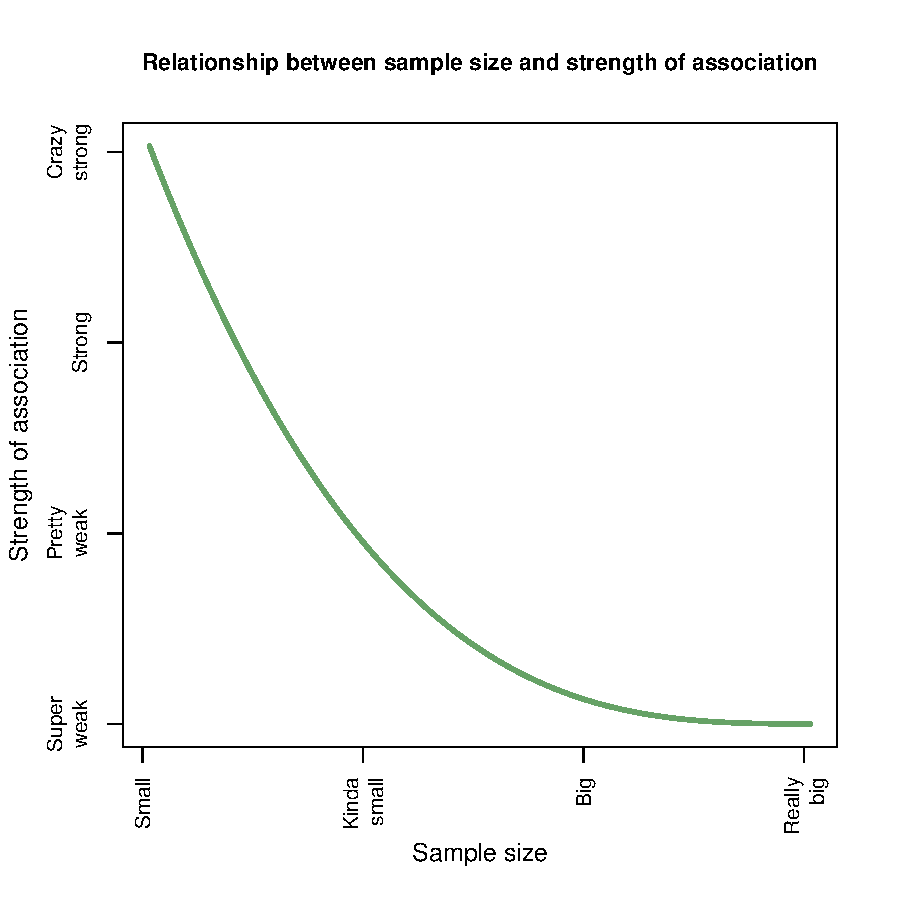
\includegraphics{hw4_brew-001}
\end{center}

See \href{https://analystinstitute.org/power-calculator/}{HERE} for an interactive application related to sample size (I made it for some political work I do)..


%------------------------------------------
\subsection*{3. Effect size for own project}
\addcontentsline{toc}{subsection}{3. Effect size for own project}
%------------------------------------------

\emph{Using your own research, try to develop an outcome and predictor variable. From these variables, try to roughly estimate an effect size for your "study".}

\lettrine[nindent=0em,lines=3]{F}{or} my own research I have the weight-for-height Z-scores of approximately 1,400 Alachua first-graders, of which about 720 are white and 520 are black.  At 80\% power and with a threshold probability (p) of 0.5, I'll be able to detect a different in WHZ of 0.161.\cite{dcr}



\end{multicols}
\setkeys{Gin}{width=1\textwidth}
%----------------------------------------------------------------------------------------
%  REFERENCE LIST
%----------------------------------------------------------------------------------------
\newpage
\bibliographystyle{unsrtnat}
\bibliography{bibliography}

%------------------------------------------
\section*{Details}
\addcontentsline{toc}{section}{Details}
%------------------------------------------
%\hrulefill
%\vspace{10mm}

Full code at \href{https://github.com/joebrew/uf/tree/master/phc7000}{https://github.com/joebrew/uf/tree/master/phc7000}. \\

This report was generated on \today.  The author used R version 3.1.1 (2014-07-10) (Sock it to Me) on a mingw32 OS.  \\

The analysis in this report was written in the R programming language, and the report production was programmed in \LaTeX{} using Sweave.\\

\end{document}
